\documentclass[12pt]{article}

\usepackage{fullpage}
\usepackage{graphicx}
\usepackage{graphics}
\usepackage{mdwlist}
\usepackage{algorithm}
\usepackage{algorithmic}

% christos: these look closer to NSF specs\dots
\setlength{\oddsidemargin}{0.0in}
\setlength{\evensidemargin}{0.0in}
\setlength{\textwidth}{6.5in}
\setlength{\headheight}{0.0in}
\setlength{\topmargin}{0.0in}
% \setlength{\textheight}{9.0in}
\setlength{\textheight}{9in}
\addtolength{\textheight}{-\topmargin}
\addtolength{\textheight}{-\headheight}
\addtolength{\textheight}{-\headsep}
\addtolength{\textheight}{-\footskip}



\begin{document}

\newcommand{\beq}{\begin{equation}}
\newcommand{\eeq}{\end{equation}}
\newcommand{\bit}{\begin{itemize*}}
\newcommand{\eit}{\end{itemize*}}
\newcommand{\goal}[1]{ {\noindent {$\Rightarrow$} \em {#1} } }
\newcommand{\hide}[1]{}
\newcommand{\comment}[1]{ {\footnotesize {#1} } }
\newtheorem{lemma}{Lemma}
\newtheorem{theorem}{Theorem}
\newtheorem{proof}{Proof}
\newtheorem{defn}{Definition}
\newtheorem{algo}{Algorithm}
\newtheorem{observation}{Observation}

\title{Concrete Graph Mining: a Database approach}


\author{ {\em Wei Chen} \\
	    Dept. of Computer Science \\
	    CMU\\
	    {\tt weichen1@andrew.cmu.edu}
	 \and
	 {\em Siping Ji} \\
	     Dept. of Computer Science \\
	     CMU\\
	     {\tt sipingji@cmu.edu}
        }


\maketitle
\begin{abstract}
    How similar are two sound-clips?
what is the best rhetorical question you can ask?
In this project, we develop {\em SomeMETHOD},
a fast and effective way of measuring the similarity
between two short sound clips.

\end{abstract}

\section{Introduction}
    \label{sec:intro}
    % {\em
% \bit
% \item
% what is the problem
% \item
% what are the applications
% \eit
% }

The problem we want to solve is the following:
\bit
\item GIVEN: a graph stored as edge list in RDBMS
\item FIND: hidden patterns in this graph using various graph mining algorithms implemented by SQL language
\item to MINIMIZE: the computational cost.
\eit

With the growth of computer network, graphs are ubiquitous nowadays, social networks, papers citing network, world wide web to a few. On the other hand, with the drastic drop of storage cost and the emergence of large social network companies like Facebook and Linkedin, graphs are now of a unprecedented size with billions of vertexes and edges. Mining such large dataset may help us gain lots of useful information and leads to interesting applications anomaly detection, social network analysis and so on. There are also lots of famous graph mining algorithms like PageRank, Random Walk with Restart, Belief Propagation who are aiming to find interesting patterns in graphs. However, most of these algorithms assume the graph fit in memory, which is apparently no longer suitable for the giant graphs today.

In this paper, we focus on how to use SQL language to implement efficient graph mining algorithms to find interesting patterns in large graphs that are stored in relational databases. We want to justify that RDBMS, equipped with highly optimized query engine and in-memory index, is sufficient for us to develop efficient and scalable graph mining algorithms in order to deal with graphs in this big data era.  

% The contributions of this project are the following:
% \bit
% \item our proposed {\em someMETHOD} is novel, combining wavelets
%       with a spike-removal  preprocessing step
% \item it is effective, achieving 90\% classification accuracy
% \item it is scalable, being linear on the number of sound-clips $N$.
% \eit


\section{Survey}
    \label{sec:survey}
    Next we list the papers that each member read,
along with their summary and critique.

% Table \ref{tab:symbols} gives a list of common symbols we used.
% \begin{table}[htb]
% \begin{center} 
% \begin{tabular}{|l | c | } \hline \hline 
% Symbol & Definition \\ \hline
% $N$ & number of sound-clips \\
% $D$ & average duration of a sound-clip \\
% $k$  & number of classes \\ \hline
% \end{tabular} 
% \end{center} 
% \caption{Symbols and definitions}
% \label{tab:symbols} 
%  \end{table} 

\subsection{Papers read by Siping Ji}
The first paper was the wavelet paper by Kang
\cite{Kang09}
\begin{itemize*}
\item {\em Main idea}: 
		This paper proposes a parallel programming primitive GIM-V that captures the shared characteristics among many seemingly different graph mining algorithms. The key idea is that the computation of graph mining algorithms like Pagerank, RWR, diameter estimation and so on, are essentially iterations of a generalized matrix-vector multiplication. More specifically, this generalized matrix-vector computation step can be captured by three basic operators in GIM-V - combine2, combineAll and assign. Based on this abstraction, many graph mining algorithms can be effciently computed via GIM-V over hadoop. Further, the author addresses the problem of high computational overhead of the shuffling stage in map-reduce. To overcome the problem and thus enhance the scalability, the author introduces several techniques, namely blocking, edge-clustering, diagonal block iteration and node renumbering into the implementation of GIM-V.
\item {\em Use for our project}:
      Although GIM-V is a hadoop-based implementation, it is still a good reference for us since matrix-vector multiplication is easy to implement under SQL.  We can also implement the operator primitives of GIM-V(combine2, combineAll and assign) using user-defined function in PostgreSQL.

\item {\em Shortcomings}:
      
\end{itemize*}
The second paper was by Kang
\cite{DBLP:conf/icdm/KangMAF10}
\begin{itemize*}
\item {\em Main idea}: 
		This paper studies and analyzes the patterns in connected components in real world large graphs. By introducing the concept of Graph Fractal Dimension(GFD) as a measure of the density of a connected component and the maximum effective radius(MER) vs. average effective radius(AER) ratio, the author shows there exists both consistency and difference among connected components of different size. Besides, the author also suggests an log-linear relationship between rebel probability of a newcomer node and its degree in dynamically evolving graphs. Based on these observations, the author proposes a Community Connection model to explain the growth process of a graph and justifies that this model correctly captures the patterns they discovered.

\item {\em Use for our project}:
      It is very relevant to the task of implementing the connected component algorithm. Additionally, this paper exemplifies how to discover, analyze and model the hidden pattern in a graph instead of treating statistics only as useless numbers. I think this helps us better explain the result in our experiment process.

\item {\em Shortcomings}:
	Though this paper discusses extensively about analyzing and model patterns of connected components of a graph, it doesn’t address much about how to apply this pattern and model to applications. Also, the implementation detail of finding connected components is ignored in the paper, which is what our project mainly focuses.

\end{itemize*}

The third paper was by Kang
\cite{kang2010inference}
\begin{itemize*}
\item {\em Main idea}:  
		Belief Propagation(BP) is an popular graphical model algorithm for inferring the states of nodes in Markov Random Fields, it has been successfully applied to many problems in the fields of social network analysis, computer vision and so on. There already exists many efficient BP algorithms, but all of them assumes the graph can fit in main memory. This paper addresses exactly the problem of how to scale up the belief propagation(BP) algorithm to giant graphs with billions of nodes that can only stored on disks. The author first proposes the GIM-V - a primitive for parallel graph mining algorithms based on hadoop. It is based on the observation that the computation process of many existing graph mining algorithm like pagerank, random walk with restart are essentially repeated matrix vector multiplication by customizing the sub-operations in a matrix multiplication. Next, the author shows that by converting the original graph to a directed line graph, the key step in the BP computation that updates the messages vectors can be viewed as a process of matrix-vector multiplication, and thus can be applied to the framework of GIM-V. To further improve the efficiency of the parallel computing algorithm, the author introduces a trick of lazy multiplication to reduce the computation cost of multiplication operations. In the experiment, it shows that the method proposed beat the single machine BP algorithm in terms of running time, and when the number of machines increases, the algorithm scales up near linearly.

\item {\em Use for our project}:
       Although the algorithm proposed in this paper is based on hadoop, it's still insightful to see the reinterpretation of the process of computing BP as a matrix-vector multiplication step. This insight may inspire us to efficiently compute BP in RDBMS, since the computation of sparse matrix-vector multiplication can be very efficient due to highly optimized query execution and in-memory index.
\item {\em Shortcomings}:
		The major weakness of this paper is that it only compare their method to single-machine BP algorithm. It also lacks the theoretic justification for the near-liner scalability of their algorithm.
\end{itemize*}

\subsection{Papers read by Wei Chen}
The first paper was "Mining Large Graphs: Algorithms, Inference, and Discoveries".
\cite{DBLP:conf/icde/KangCF11}
\begin{itemize*}
\item {\em Main idea}: 
This paper discuss how to do inference in graphical model under distributed setting, what if graph can not fit into main memory. They propose a variant of Belief Propagation called \emph{Line Graph Fixed Point(LFP)} to address this issue. The key step is to induce a new graph called \emph{Directed Line Graph} L(G) from original graph, it flips the definition of node and edge. Each node of L(G) represents an edge of G and edge exists between node $n_{i}$ and $n_j$ if and only if their related edges are incident. L(G) has a nice property that it's easy to derive exact recursive equation for it, actually the message updating equation of original Belief Propagation \cite{bp} can be adopted without modification. Then the author generalize mesage updating procedure as general Matrix-Vector operations, namely combine2(), combineAll(), sumVector() and assign() from \cite{Kang09}. While directly apply LFP without careful design will lead to drastic storage requirement to store L(G), the idea to tackle this is \emph{Lazy Multiplication}, all operations on L(G) is is actually run on G. They propose an algorithm employing this idea, and run on Hadoop, its name is \emph{Hadoop Line Graph Fixed Point}. Ha-LFP solves the biggest issue of the most graph mining algorithm --- scalability. Since Ha-LFP is based on Hadoop, it inherits fault tolerance, data replication natively.
\item {\em Use for our project}:
      LFP seems like a promising method to do Belief Propagation, combine2, combineAll, assign is natural in SQL. Matrix operation is tractable in SQL, and can be optimized by RBDMS. The performance could be comparable to Hadoop version. Also we don't need to construct L(G) explicitly, this avoids expensive cost in storage and time to access and update L(G).
\item {\em Shortcomings}:
      It's kind of tricky to say this algorithm solve scalability perfectly. I think this is more contributed to Hadoop instead of LFP. There may exist better formulation of Belief Propagation on Hadoop. The experiments are conducted on M45, which is one of the most advanced supercomputer.
\end{itemize*}


The second paper was "Understanding Belief Propagation and its Generalizations".
\cite{bp}
\begin{itemize*}
\item {\em Main idea}: Marginal Probability is important in graphical model inferencing, while most of the time it is expensive to calculate, the running time is usually exponential to the number of nodes. \emph{Belief Propagation} is a neat technique to bring the running time down to linear to the number of edges in graphical model, and it has been widely used beyong machine learning, like computer vision\cite{felzenszwalb2006efficient}, turbo code 
\cite{mceliece1998turbo}, etc. The success of Belief Propagation results from a property called \emph{Conidtional Independence}. Most graphical models have the property that there exist many conditional independence between nodes. The core idea of Belief Propagation is to exploit this property to decouple the computation of global probability into several load computations. The marginal probability of node $n_{i}$ is called \emph{belief}. Each node $n_{i}$ sends messages to other nodes $n_{j}$. \emph{Message} $m_{ij}(n_{j})$ represents how node $n_{i}$ thinks node $n_{j}$'s state should be. A node can calculate its belief once it has received messages from all its neighbouts. So each edge is associate with two messages. The paper shows that each message can be calculated only once, thus we can use dynamic programming to compute every node's belief in linear time. The paper also introduce Generalized Belief Propagation which extends BP to group of nodes.
\item {\em Use for our project}:
      This paper discusses how to compute belief of each node in one round(for trees). We can first implement the algorithms mentioned in this paper as a baseline. It is also helpful for understanding other optimizing algorithms for Belief Propagation. 
\item {\em Shortcomings}:
       There is not much discussion about the implementation in SQL. But user defined functions provided by PostgreSQL has limited expressiveness, so the real implementation will be quite different.
\end{itemize*}


The third paper was "A Comparison of Approaches to Large-Scale Data Analysis".
\cite{pavlo2009comparison}
\begin{itemize*}
\item {\em Main idea}: 
    This paper compares the tradeoff between Parallel DBMS and MapReduce framework in large data analysis. The authors want to advocate the capability of Parallel DBMS in implementing large scale analytic tasks. The paper analyze the fundamental difference of Parallel DBMS and MapReduce, their support in schema, data distribution, fault tolerance, index, and utility tools. Then they conduct experiments about their performance in different tasks, like pattern searching, aggregation, join, etc. They conclude that Parallel DBMS outperforms MapReduce in all kinds of tasks. But Parallel DBMS requires a lot of effort to configure and profile to reach good performance, MapReduce is relatively much easier to use. In the end, the paper admit MapReduce's advantage over complex Parallel DBMS, while still suggest Parallel DBMS as an option for specific tasks.
\item {\em Use for our project}:
    We can borrow some ideas from theirs experiments about investigate SQL function. Their analysis method is also a good model to follow.
\item {\em Shortcomings}:
    The tasks they experimented are kind of trivial. We don't know the real difference in when the systems are used for more complex graph mining algorithms.
\end{itemize*}

The fourth paper was "Pig Latin: A Not-So-Foreign Language for Data Processing".
\cite{olston2008pig}
\begin{itemize*}
\item {\em Main idea}: 
    Either RDBMS or MapReduce framework represents some extreme in large scale data analysis, either unnatural for programmers' mind(SQL) or too low level to express many algorithms(MapReduce). Different solutions are proposed. Pig is a platform of Yahoo that try to reach a balance between these two styles to support more flexible(ad-hoc) data analysis tasks. It takes a hybrid strategy, provides friendly user interface(programming, debugging), while actual tasks are running on powerful Hadoop platform without loss of performance. And it propose a new high level programming language called \emph{Pig Latin} that gives user more control of data flow, which programmer can adopt an imperative style, while retain the expressiveness of SQL. It also support several key operations that can be automatically parallelized, like filter, cogroup, group, join, etc. Its underlying implementation is compile Pig Latin programs into Hadoop jobs, so that it is also equipped with the benefits of MapReduce. 
\item {\em Use for our project}:
    Pig Latin's SQL-like syntax provides finer grained control over dataflow, which is more suitable for implementing graph mining algorithms. We can compare with SQL user defined function implementation of these algorithms, and analyze their intrinsic data accessing characteristic.
\item {\em Shortcomings}:
    There are few graph mining algorithms implementation in Pig Latin, only a few open source analysis package like Linkedin's Datafu. And Pig only supports read-only data analysis workloads, which may lead to many unnecessary efforts if we want to do extensive write during computation.
\end{itemize*}


\section{Proposed Method}
    \label{sec:proposed}
    We implement all the graph mining algorithms using Postgres's embedded PL/pgSQL programming language, which supports many advanced features, like user defined function, aggregate, etc. It also has a sophisticated query execution engine, which we think is the most critical component of Postgres.

The following are the algorithms we plan to implement. The reason we choose them is that there are a lot of implementation in other platform like MapReduce, we can compare our SQL version with them to draw a clusion about SQL's unique charastic in solving data analytic tasks.

\begin{description}
  \item[PageRank:] Determine the importance of every node of a graph based on its connectivity. 
  \item[Connected Components:] Partition the nodes of a graph also based on its connectivity.
  \item[Radius of Every Node:] Compute the radius of every node in a graph. The radius is defined as the number of hops that a node needs to reach to its furthest neighbor.
  \item[Belief Propagation:] Calculate the marginal probability of each node in a graphical model. 
  \item[Eigenvalue:] Using approximation method to estimate the top-k eigenvalues of a matrix.
\end{description}

\subsection{Pagerank}
The algorithm of pagerank is Power method. We do matrix multiplication continusly until the change in pagerank is small. 
\begin{algorithm}
\caption{Pagerank}
\begin{algorithmic}
\STATE{Bulk load graph into an edge table in database.}
\STATE{Initialization(damper factor=0.85, max iteration = 100, epsilon = 0.0001)}
\STATE{Build a weight matrix trans, initialize pagerank p}
\REPEAT
\STATE{For each node i, update its pagerank with its old value and its income node's pagerank.}
\UNTIL{Convergence}
\end{algorithmic}
\end{algorithm}

\subsection{Weakly connected components}
In terms of the implementation of weakly connected components. We borrow the idea of HCC method from the "PEGASUS" paper.\cite{Kang09}
The algorithm can be described as following:
\begin{algorithm}
\caption{Weakly Connected Component}
\begin{algorithmic}
\STATE{Bulk load graph into an edge table in database.}
\STATE{Create a component table, where each entry contains a node id, and the component id.}
\STATE{Initialize the component table where component id equls node id.}
\REPEAT
\STATE{For each node, assign the minimum component id of its neighbors as the new componnet id of this node.}
\UNTIL{Convergence}
\end{algorithmic}
\end{algorithm}
After several rounds of iteration, the nodes in the same connected component will share the same component id.
The number of iterations for convergence can be proved to be upper bounded by the diameter of the graph.

\subsection{Radius of every node}
We discard the traditional algorithm because it is extremely infeasible for large graphs, since it uses a set to record every neghbors within n hops for a node during iteration, which requires a O($n^2$) space.
Since the exact algorithm is hopeless, we use the approximation algorithm described in "HADI" paper\cite{DBLP:journals/tkdd/KangTAFL11} instead. Specifically, we use the Flajolet-Martin algorithm for counting the number of distinct members in a multiset. It is guaranteed to give an unbiased estimate and a tight O($log(N)$) bound for space complexity. The basic idea of Floajolet-Martin algorthm is to use a bitstrings of length $L$ to encode the set. For each element to add, we randomly pick up a index according to a specified distribution, and assign BITMAP[index] to 1. Following this procedure to add element, the size of the final set can be estimated by $\frac{1}{\phi} 2^{\frac{1}{k}\sum_{i=1}^k R_i}$, where $\phi$ = 0.77351, $R_i$ denotes the index of the leftmost 0 in the the $k$th bitstring.

In our proposed method for computing radius of every node, we use the Flajolet-Martin(FM) bitstrings to encode the neighbors of every node. Formally, we use $k$ FM-bitstrings $b(h, i)$ to represent the set of neighbor nodes reachable from $node_i$ within h hops. And for each iteration, we use the following way to update each FM-bitstring:$$b(h,i) = b(h-1,i)  \quad BIT-OR \quad  {b(h-1,j)|(i,j)\in E}$$

Given the above description of how to encode neighbors of a node, and the method to update bitstrings, we can describe the approximation method we used to compute the raidus of every node in algorithm \ref{radius:algo3}.

\begin{algorithm}
\caption{Radius of Every Node}
\begin{algorithmic}
\STATE{Bulk load graph into an edge table in database.}
\STATE{Preprocess the edge table, add a self loop edge to every node in the graph.}
\STATE{Intialize the vertex table, which contains node id, and a column of bitstring array, the bitstrings are initialized using the FM algorithm}
\REPEAT
\STATE{For every node update the bitstring according to formula: $b(h,i) = b(h-1,i) \quad BIT-OR \quad  {b(h-1,j)|(i,j)\in E}$. }
\STATE{For every node, check whether the bitstrings is unchanged before and after updates, if it's not changed, output i as the radius for this node.}
\UNTIL{The bitstrings of every node stablizes or it reaches the maximum rounds of iteration.}
\end{algorithmic}
\label{radius:algo3}
\end{algorithm}


To make this algorithm possible in SQL, we defined some user defined functions:
\begin{description}
  \item[fmAssign:] Assign the k FM-bitstrings for a node.
  \item[bitOr:] Execute the OR operations between two bitstring arrays.
  \item[aggBitOr:] Aggregate function for bitOr.
  \item[fmSize:] Estimate the size of a set encoded by FM-bitstring.
\end{description}

\subsection{Belief Propagation}
For belief propagation, we use the fabp method proposed in paper\cite{DBLP:conf/pkdd/KoutraKKCPF11}.
It can be shown that the solution of belief propagation can be approximated by the linear system:$$[\mathbf{I}	 + a\mathbf{D} - c\mathbf{A}]\mathbf{b_h} = \mathbf{\phi_h}$$ 
where $\mathbf{A}$ is the n by n symmetric adjacency matrix, $\mathbf{D}$ is the diagonal matrix of degrees, $b_h$ corresponds to the vector of final beliefs for each node, $\phi_h$ is prior belief vector, and $h_h$ is the homophily factor,  $a = 4h_h^2/(1 - h_h^2)$ and $c = 2h_h / (1-4h_h^2)$.

To solve this linear system, we can see :$\mathbf{I} + a\mathbf{D} - c\mathbf{A}$ as the form $\mathbf{I} - \mathbf{W}$, where $\mathbf{W} = -a\mathbf{D} + c\mathbf{A}$, and using the expansion:$$(\mathbf{I} - \mathbf{W})^{-1} = \mathbf{I} + \mathbf{W} + \mathbf{W}^2 + \mathbf{W}^3 + ...$$

and the solution of the linear system is given by the formula:
$$\mathbf{b_h} = (\mathbf{I} - \mathbf{W}^{-1})\mathbf{\phi_h} =\mathbf{\phi_h}  + \mathbf{\phi_h} \mathbf{W} + \mathbf{\phi_h} \mathbf{W}^2 + \mathbf{\phi_h} \mathbf{W}^3 + ...$$

Given this power method, the implementation is pretty straightforward as described in algorithm \ref{bp:algo4}.
\begin{algorithm}
\caption{Belief Propagation}
\begin{algorithmic}
\STATE{Bulk load graph into an edge table in database.}
\STATE{Initialize $h_h = 0.001 $}
\STATE{Initialize the initial belief of every node as prior belief}
\REPEAT
\STATE{Update the belief of node by $b_h(i) = b_h(i-1)\mathbf{W} + \mathbf{\phi_h}$ }
\UNTIL{Convergence}
\end{algorithmic}
\label{bp:algo4}
\end{algorithm}

\subsection{Eigenvalue/SVD}
We adopt the method propose in \cite{kang2011spectral}. There are several methods to solve part of eigenvalue computation problems, for instance, power method\cite{langville2004deeper}. While it has the limitation that it can only extract the eigenvector with biggest eigenvalue. Several method have been proposed to extract top k eigenvectors simultaneously. The approach we use is Lanczos algorithm\cite{lanczos1950iteration}. The general idea about this algorithm is that instead of directly work on an $N \times N$ matrix, we first generate a skinny $N \times m$ matrix(M $\ll$ N). Then it computes a small $M \times M$ dense matrix which has good approximation to the eigenvalues of the original matrix. In this case, we directly apply quadratic algorithm to top-k eigenvalues. Notice that k $<$ M.

{\bf{Algorithm detail:}} Different from power method, the intermediate multiplication matrix is used to construct a set of orthonormal base of \emph{Krylv subspace $K_{m}$} which follows the definition:
\begin{equation}
K_{m} = < b, Ab, \cdots, A^{m-1}b>.
\end{equation}
The sub procedure to construct orthonormal bases may be any standard algorithm, for example Gram-schmidt algorithm. We can view Lanczos algorithm as an iterative method which incrementally construct Krylov subspace. The pseudo-code is shown in Algorithm \ref{eigen:algo1}.

After Lanczos factorization, we get a few matrices that satisfy the following equation:
\begin{equation}
	AV_{m} = V_{m}T_{m} + f_{m}e^{T}_{m}
\end{equation}
To name a few, $A^{n\times m}$ is input matrix, $V^{n\times m}_{m}$ contains the m orthonormal bases, $T^{m\times m}_{m}$ is a tridiagonal matrix, $f_{m}$ is new n-vector orthogonal to all columns of $V_{m}$, $
e_{m}$ is a vector that \emph{m}th element is 1, and others 0. After algorithm \ref{eigen:algo1}, we need to construct the matrix $T^{m\times m}_{m}$. The algorithm is quite simple, it is listed in algorithm \ref{eigen:algo2}. 

The eigenvalues of $T_{m}$ are called Ritz values, and $V_{m}Y$'s columns are called Ritz vector. It is constructed by Algorithm \ref{eigen:algo3}. We expect the Ritz values and Ritz vectors to be good approximation of the eigenvalues and eigenvectors of original matrix. The computation of eigenvalues of $T_{m}$ can be done by standard quadratic algorithms, such as QR method. 

\begin{algorithm}
{\bf Input:} Matrix $A^{n \times m}$\\
random n-vector $b$,\\
number of steps m\\
{\bf output:} Orthogonal matrix $ V^{v \times m}_{m} = [v_{1}\cdots v{m}]$,\\
coefficients $\alpha[1..m]$ and $\beta[1..m-1]$
\begin{algorithmic}[1]
\caption{Lanczos algorithm}
\STATE $\beta_{0} \leftarrow 0, v_{0} \leftarrow 0, v_{1} \leftarrow \frac{b}{\parallel b \parallel}$ 
\FOR {$i=1$ to $m$}
	\STATE $v \leftarrow Av_{i}$
	\STATE $\alpha_{i} \leftarrow v^{T}_{i}v $
	\STATE $v \leftarrow v - \beta_{i-1}v_{i-1} - \alpha_{i}v_{i}$
	\STATE $\beta_{i} \leftarrow \parallel v\parallel $
	\IF {$\beta_{i} = 0$} 
	\STATE break for loop 
	\ENDIF
	\STATE $ v_{v+1} \leftarrow \frac{v}{\beta_{i}} $
\ENDFOR
\end{algorithmic}
\label{eigen:algo1}
\end{algorithm}

\begin{algorithm}
\caption{Build tridiagonal matrix}
{\bf Input:} $\alpha, \beta$
{\bf Output:} $T^{m\times m}_{m}$
\begin{algorithmic}[1]
\FOR {$i=1$ to m}
	\STATE $T[i, i] \leftarrow \alpha_{i} $
	\STATE $T[i, i+1] = T[i+1, i] \leftarrow \beta_{i}$
\ENDFOR	
\end{algorithmic}
\label{eigen:algo2}
\end{algorithm}

\begin{algorithm}
\caption{Compute Ritz values}
{\bf Input:}Orthogonal matrix $V^{n\times m}_{m}$\\
coefficients $\alpha[1..m]$ and $\beta[1..m-1]$
\begin{algorithmic}[1]
\STATE $T_{m} \leftarrow$ (build a tridiagonal matrix from $\alpha$ and $\beta$)
\STATE $QDQ^{T} \leftarrow EIG(T_{m})$
\STATE $\lambda_{1..k} \leftarrow$ (top k eigenvalues from D)
\STATE $Q_{k} \leftarrow $ (k columns of Q corresponding to $\lambda_{1..k})$
\STATE $R_{k} \leftarrow V_{m}Q_{k}$
\end{algorithmic}
\label{eigen:algo3}
\end{algorithm}

\subsection{Minimum Spanning Tree}
We use the classical Prim's algorithm for this additional task. We abandon the Kruskal's algorithm because the disjoint set is not easy to implement using SQL. The implementation can be described in algorithm \ref{prim:algo}.

\begin{algorithm}
{\bf Input:} Edge Table E of a undirected connected graph \\
{\bf output:}  Edge Table MST containing edges of the minimum spanning tree
\begin{algorithmic}
\caption{Prim's algorithm}
\STATE Create a node table N$ 
\STATE Randomly insert a node into N
\FOR {$i=1$ to $number of nodes - 1$}
	\STATE Insert into MST an edge from E with minimum weight where src node is in N and destination node is not in N
	\STATE Insert into N with the destination node of the edge selected in last step
\ENDFOR
\end{algorithmic}
\label{prim:algo}
\end{algorithm}







\section{Experiments}
    \label{sec:experiments}
    \subsection{Dataset}
We have conducted experiments on the following datasets(Mainly For Phase 1):
\begin{center}
\begin{tabular}{| l | c |}
  \hline                        
  Dataset Name & Advogato  \\ \hline
  Largest conn compo & 5054  \\ \hline
  Size & 6551 vertices  \\ \hline
  Volume & 51332 edges \\ \hline
\end{tabular}
\end{center}

In out final experiment suit, a more large and diverse datasets from different domains will be explored. The tentative source of experiment dataset are listed below:
\begin{description}
	\item{{\bf SNAP:}}{It has abundant data about social network, we plan to conduct triangle counting, pagerank, radius computing experiment which will reveal the underlying feature of large graphs and spot strange graphs.}
	\item{{\bf Konect:}}{Konect has more diverse datasets compared to SNAP, like citation network. It's a good target to analyze features of non-social networks, we will examine whether such networks follow power law by generating degree distribution, etc.}
\end{description}

We also calculated statistics about the weakly connected components in table \ref{table:wcc}.We compute radius for every node in Advogato dataset, the result is in table \ref{table:radius}:

\subsection{Task 1: Degree distribution}

\subsubsection{Description}
We conduct 5 experiments on large scale graph data(all with more than 1 million nodes). The details of each dataset is as follows: \\

\begin{center}
\begin{tabular}{| c | c | c |}
    \hline
    name & nodes & edges \\ \hline
    Roadnet-ca & 1,965,206 & 5,533,214 \\ \hline
    Roadnet-PA & 1,088,092 & 3,083,796 \\ \hline
    Roadnet-TX & 1,379,917 & 3,843,320 \\ \hline
    wiki-Talk & 2,394,385 & 5,021,410 \\ \hline
    Youtube & 1,134,890 & 2,987,624 \\ \hline
\end{tabular}
\end{center}


Following(Figure \ref{t1:plot}) are the rank-frequency plots of each dataset, (a)(b) shows the in degree and out degree out Wikitalk. (c) is Roadnet-Ca. (d) is Roadnet-PA. (e) is Roadnet-TX. (f) is Youtube. 

\subsubsection{Plots}

\begin{figure}[!htbf]
\begin{center}
\begin{tabular}{c c c}
     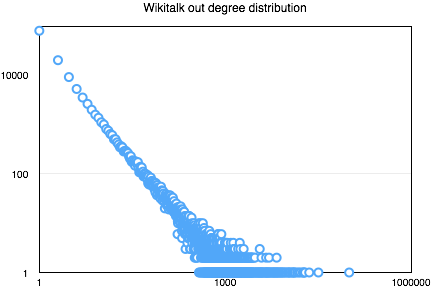
\includegraphics[width=0.3\textwidth]{FIG/t1_wiki_in.png} &
     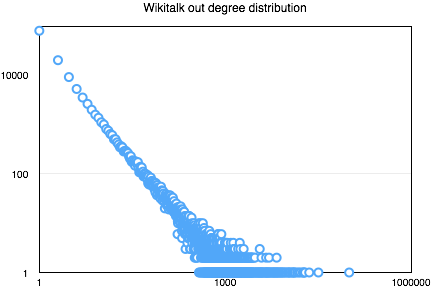
\includegraphics[width=0.3\textwidth]{FIG/t1_wiki_out.png} & 
     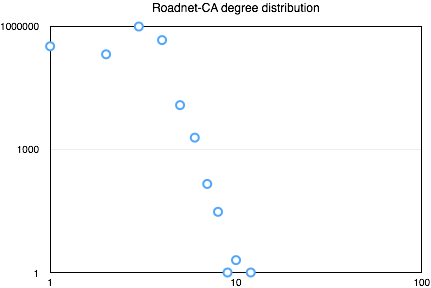
\includegraphics[width=0.3\textwidth]{FIG/t1_ca.png}\\
    (a) & (b) & (c) \\
     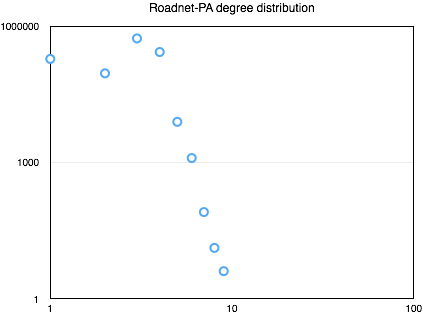
\includegraphics[width=0.3\textwidth]{FIG/t1_pa.png} & 
     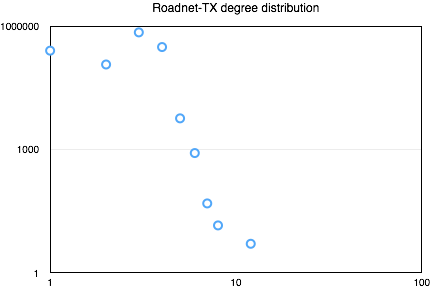
\includegraphics[width=0.3\textwidth]{FIG/t1_tx.png} & 
     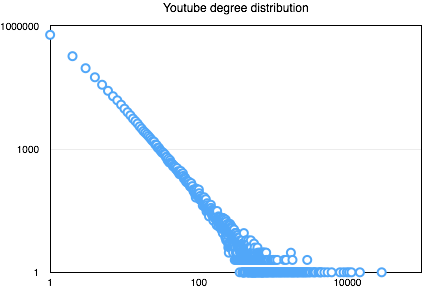
\includegraphics[width=0.3\textwidth]{FIG/t1_youtube.png} \\
     (d) & (e) & (f) \\
\end{tabular}
\caption{In degree distribution (a) and out degree distribution (b) of Wikitalk (c) Roadnet-CA, (d) Roadnet-PA (e) Roadnet-TX (f) Youtube}
\label{t1:plot}
\end{center}
\end{figure}

\subsubsection{Observation}
As we can observe, that most \emph{social network} exhibit perfect power law in degree distribution. It aligned with our intuition. While for the series of Roadnet dataset, we can not observe obvious power law. So maybe we can conclude that not all graphs have power law property in it. Some datasets like roadnet, involves a lot of human design, is less \emph{chaotic} than ordinary graphs.

\subsection{Task 2: Pagerank}

\subsection{Task 3: Weakly Connected Component}
In this experiment, we run weakly connected component in several datasets of various size.

\subsubsection{Plot}
We draw size-frequency plot in log-log scales.
\begin{figure}[h]
\begin{center}
     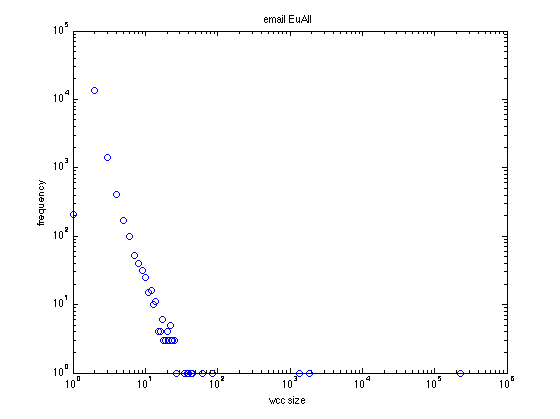
\includegraphics[width=0.8\textwidth]{FIG/t3_email_euall.png} 
\caption{Email-EuAll }
\label{t3:1}
\end{center}
\end{figure}

\begin{figure}[h]
\begin{center}
\begin{tabular}{cc}
     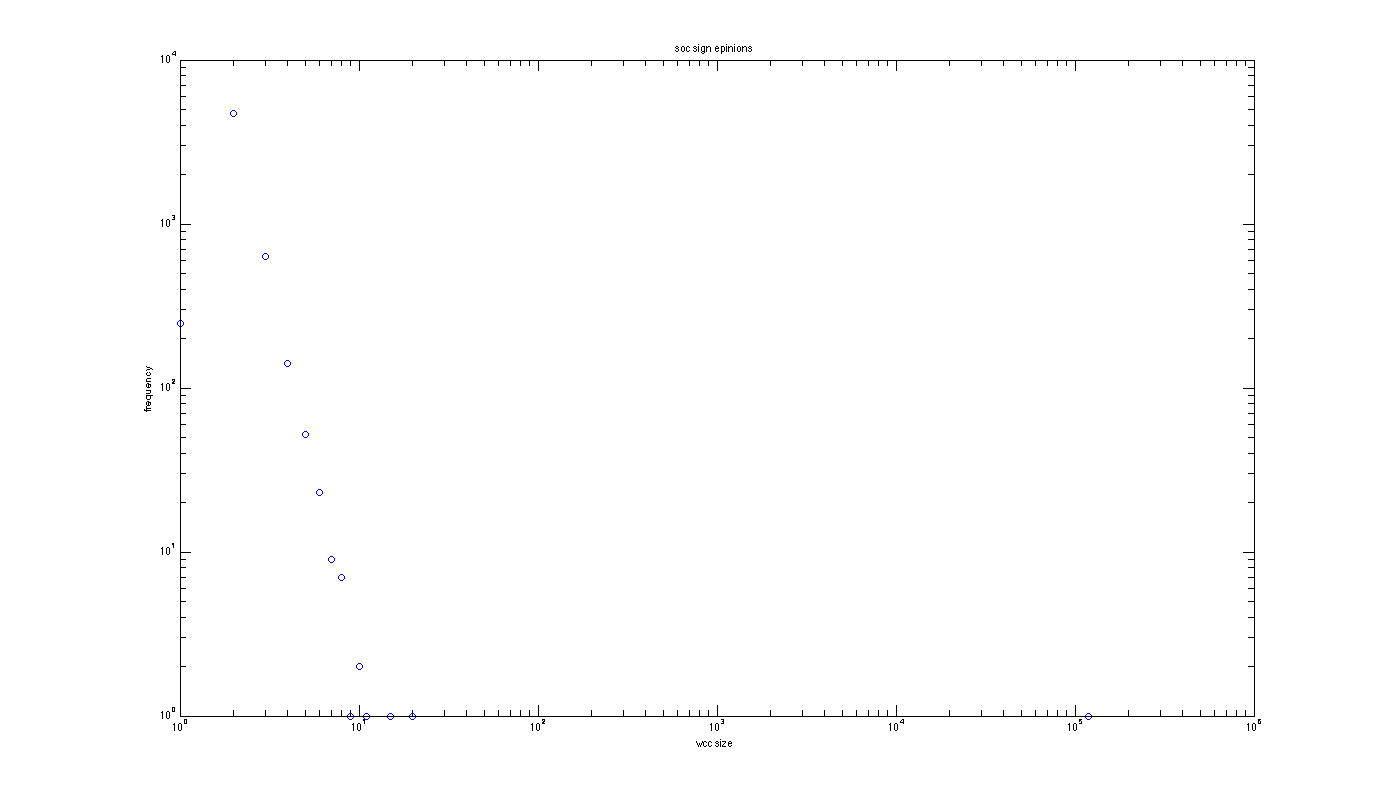
\includegraphics[width=0.8\textwidth]{FIG/t3_soc_sign_epinions.png} 
\end{tabular}
\caption{Soc-Sign-Epinions}
\label{t3:2}
\end{center}
\end{figure}


\begin{figure}[h]
\begin{center}
     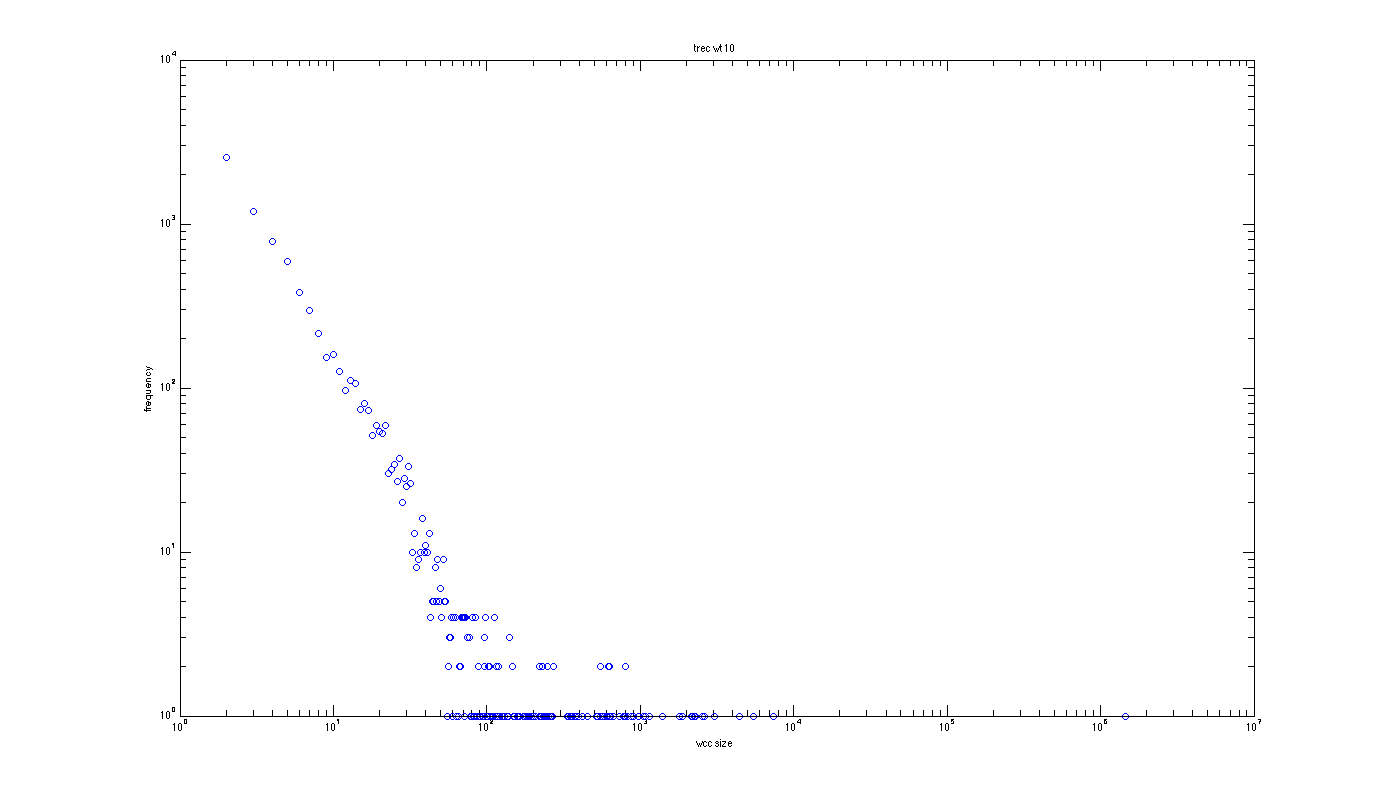
\includegraphics[width=0.8\textwidth]{FIG/t3_trec_wt10.png} 
\caption{Trec-wt10g}
\label{t3:3}
\end{center}
\end{figure}


\begin{figure}[h]
\begin{center}
     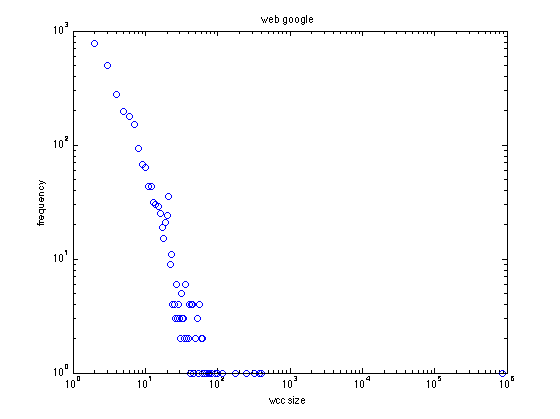
\includegraphics[width=0.8\textwidth]{FIG/t3_web_google.png} 
\caption{Google Web Graph}
\label{t3:4}
\end{center}
\end{figure}


\begin{figure}[h]
\begin{center}
     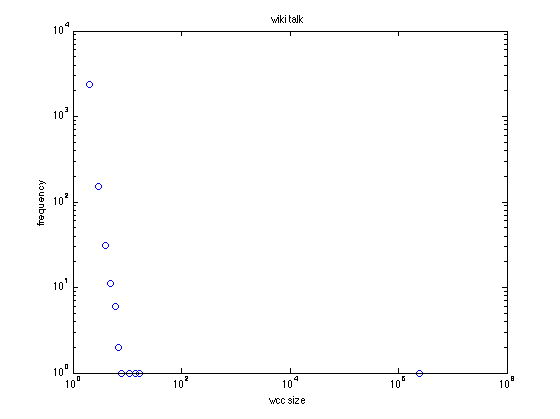
\includegraphics[width=0.8\textwidth]{FIG/t3_wiki_talk.png} 
\caption{Wiki Talk}
\label{t3:5}
\end{center}
\end{figure}

\subsubsection{Observation}
1. From the log-log scale frequency-size plot, we find that generally frequency-size follows the power law. Connected components of small sizes tend to occur more often those of larger sizes.

2. In all the plots, there is a giant connected component that contains the majority of nodes in the graph. 






\subsection{Task 4: Radius of Every Node}

\subsubsection{Experiment on large datasets}
In this experiment, we run our radius algorithm in several large datasets. The statistics of these datasets are presented in Table \ref{t4:table1}

\begin{table}[!htbf]
\caption{Datasets Statistics}
\begin{center}
\begin{tabular}{|c|c|c|c|}
\hline \hline
dataset & number of vertices & number of edges & diameter \\
\hline
DBLP co-authorship network & 317080  & 1049866  & 21  \\
Epinions social network & 131828  & 841372  & 14  \\
Amazon product co-purchasing network & 334863 & 925872 & 44 \\
EU email communication network & 265214 & 420045 & 14 \\
Google web graph & 875713 & 5105039 & 21 \\
Youtube social network & 1134890 & 2987624 & 20 \\
\hline
\end{tabular}
\end{center}
\label{t4:table1}
\end{table}%


\begin{figure}[!htbf]
\begin{center}
     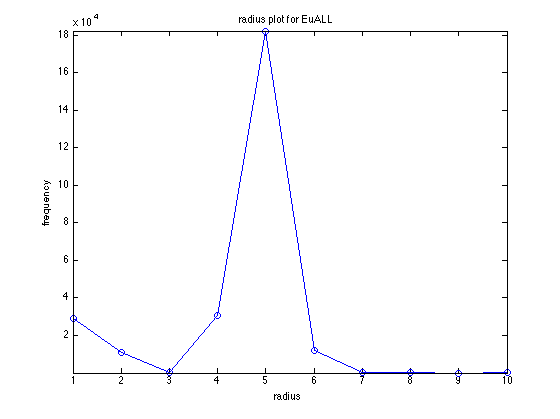
\includegraphics[width=0.8\textwidth]{FIG/t4_email.png} 
\caption{EU Email Communication }
\label{t4:1}
\end{center}
\end{figure}

\begin{figure}[!htbf]
\begin{center}
\begin{tabular}{cc}
     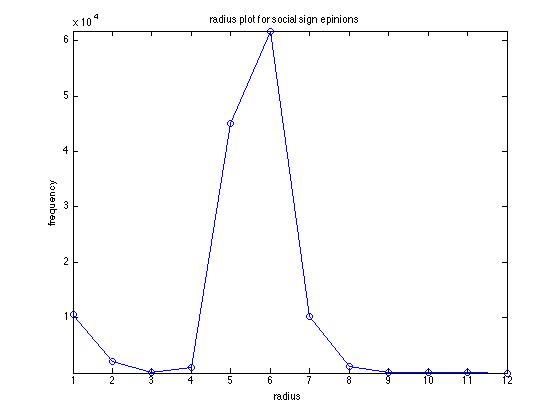
\includegraphics[width=0.8\textwidth]{FIG/t4_epinions.png} 
\end{tabular}
\caption{Epinions social network}
\label{t4:2}
\end{center}
\end{figure}


\begin{figure}[!htbf]
\begin{center}
     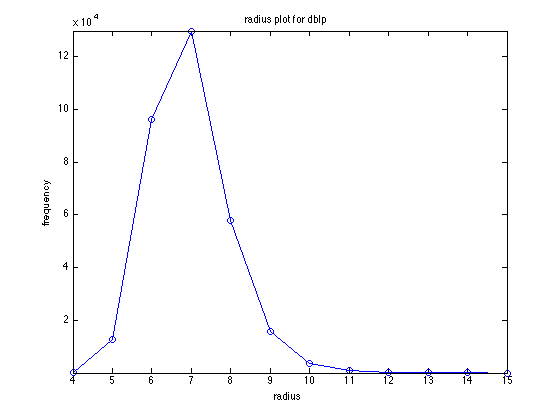
\includegraphics[width=0.8\textwidth]{FIG/t4_dblp.png} 
\caption{DBLP co-authorship network}
\label{t4:3}
\end{center}
\end{figure}


\begin{figure}[!htbf]
\begin{center}
     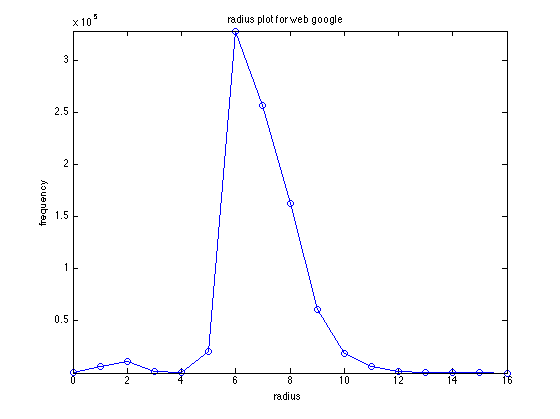
\includegraphics[width=0.8\textwidth]{FIG/t4_google.png} 
\caption{Google Web Graph}
\label{t4:4}
\end{center}
\end{figure}


\begin{figure}[!htbf]
\begin{center}
     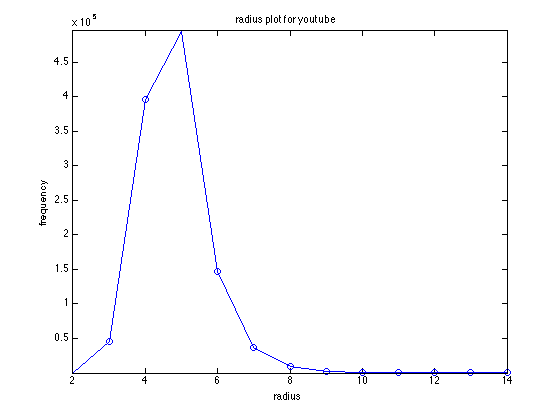
\includegraphics[width=0.8\textwidth]{FIG/t4_youtube.png} 
\caption{Youtube Social Network}
\label{t4:5}
\end{center}
\end{figure}

\begin{figure}[!htbf]
\begin{center}
     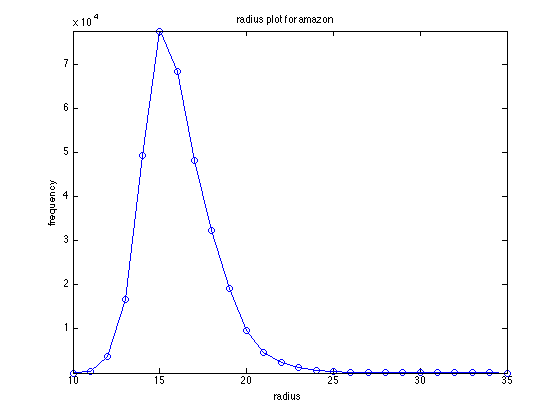
\includegraphics[width=0.8\textwidth]{FIG/t4_amazon.png} 
\caption{Amazon product co-purchasing networkk}
\label{t4:6}
\end{center}
\end{figure}


 
\subsubsection{Observation}
1. Radius Distribution: From the above plot, we find radius distribution of these graphs either tend to be single-modal, for example, EU Email Communication graph in figure \ref{t4:1} and Epinions Social Network in figure \ref {t4:2}, or bi-modal like DBLP co-authorship network in figure \ref{t4:3} and Youtube Social Network in figure \ref{t4:5}.

2. Relationship to the connected component: So why radius tend to be distributed like this, we guess it's somehow related to the connectivity of the graph. Therefore we take a look back to the statistics we got from task3. We find that the graphs that has a single-modal shape radius distribution are fully or almost fully connected. The graphs that has bi-modal radius distribution are not that well connected, For most nodes that appear in the Giant Connected Component(GCC), they tend to have a higher radius value, specifically the smaller radius value it has, the more centric it is in the GCC. On the other hand, The first peak in the radius distribution represent those disconnected components.

\subsubsection{Proof of Correctness}
Since the algorithm we use is an approximate algorithm, it's hard for us to verify the validity of our algorithm accurately. But we still try the algorithm on both small, large and synthetic datasets to demonstrate its validity.  
First we test the algorithm on the synthetic tiny dataset consisting of only 10 nodes and 8 edges. It accurately compute the radius of every node.
 
Then we test our algorithm on small datasets of several thousands of nodes, the experiment result are showed in Table \ref{table:small}, we can see that our algorithm can get a closer estimate of diameter.

\begin{table}[!htbf]
\caption{Radius Experiment on Small Datasets}
\begin{center}
\begin{tabular}{|c|c|c|c|c|}
\hline \hline
dataset & nodes & edges & real diameter & estimated diameter \\
\hline
Enron email network & 36692 & 183831 & 11 & 11 \\
High Energy Physics & 12008 & 118521 & 13 & 12 \\
Advogato Trust Network & 6551 & 51332 & 9 & 9 \\
\hline
\end{tabular}
\end{center}
\label{table:small}
\end{table}%

For large dataset we run in last section, the estimated diameter is still bounded by real diameter, but the estimation is no longer that close. This can be explained by the approximation nature of the algorithm we use. The Flajolet-Martin string we generate for every node is not unique, and as the number of nodes grows larger, the uniqueness of a node that a Flajolet-Martin string can represent is weakened. Therefore, for graph with larger size, the estimation might become less accurate.







\subsection{Task 5: Eigenvalue/Singular value}


\subsection{Task 6: Belief Propagation}

\subsubsection{Experiment on large datasets}
In this experiment, we run our radius algorithm in several large datasets. The statistics of these datasets are presented in Table \ref{t5:table1}

\begin{table}[!htbf]
\caption{Datasets Statistics}
\begin{center}
\begin{tabular}{|c|c|c|}
\hline \hline
dataset & number of vertices & number of edges \\
\hline
DBLP co-authorship network & 317080  & 1049866  \\
Epinions social network & 131828  & 841372  \\
Amazon product co-purchasing network & 334863 & 925872 \\
EU email communication network & 265214 & 420045 \\
Google web graph & 875713 & 5105039 \\
Youtube social network & 1134890 & 2987624 \\
\hline
\end{tabular}
\end{center}
\label{t5:table1}
\end{table}%

Similar to semi-supervised learning, belief propagation algorithm require the graph to be partially labeled.  However, we don't have such information. Therefore, in this experiment, we randomly assign the prior belief for all nodes. Specifically, we randomly assign 25 percent of the nodes with positive label, i.e. positive prior belief, and 25 percent of other nodes with negative label, i.e. negative prior belief, and the rest with zero belief, meaning that we don't have prior knowledge for these nodes. Then we conduct FABP algorithm on these datasets, the result are shown in Table \ref{t5:table2} .

\begin{table}[!htbf]
\caption{BP Statistics}
\begin{center}
\begin{tabular}{|c|c|c|c|}
\hline \hline
dataset & positively labeled & negatively labeled & non labeled  \\
\hline
DBLP co-authorship network & 134139  & 136636  & 46305 \\
Epinions social network & 53968  & 52796  & 25064 \\
Amazon product co-purchasing network & 143796 & 144796 & 46271 \\
EU email communication network & 100619 & 109674 & 54921 \\
Google web graph & 379568 & 376325 & 119820 \\
Youtube social network & 450084 & 457956 & 226850 \\
\hline
\end{tabular}
\end{center}
\label{t5:table2}
\end{table}%

 
\subsubsection{Observation}
1. By applying Belief Propagation algorithm on these graphs, most of the unlabeled nodes are successfully assigned either positive or negative belief.

2. We find that for some graphs, larger proportions of nodes gets labeled than other graph. For example, in DBLP co-authorship network and amazon product co-purchasing network,  about 85\%  of the nodes get labeled. While for like Epinions social network and EU emali communication network, only 75\% of the nodes get labeled. Once again, we look back at the connectivity of the graph to find the probable cause. We observed that, graph that is well connected is easier to get more nodes assigned with labels. This observation makes sense in that 'beliefs' can be easier to propagate in well connected graphs than those grape with many disconnected components.

\subsubsection{Proof of Correctness}
As mentioned it the previous section, we don't have any labels for these large datasets, therefore we verify the result according to statistics we get in the last section. We can see that the proportion with positive labels and negative labels are approximately same, which resembles the label distribution with our prior belief. 







\subsection{Task 7: Triangle Counting}
According to the algorithms in \cite{tsourakakis2008fast}, we know that the number of triangles in a network is propotional to the sum of eigenvalue of its adjency matrix, which is $\frac{\sum_{i}\lambda_{i}^{3}}{6}$. Figure \ref{t7:timedata} shows the running time of global triangle counting with regards to the size of graph. We can see that as the size of graph increases, the running time also grows nearly linearly with the size. For the largest graph, which is Roadnet-PA, it runs nearly for an hour to complete. However, the predicted result for Roadnet-PA is unsatisfactory. We conduct both global and local triangle counting, all the data is listed as follows.

\subsubsection{Plots}
Table \ref{t7:timedata} lists run time of global triangle counting. Table \ref{t7:globalpredict} lists the predicted triangle count of each dataset. Figure \ref{t7:globaltime} plots the run time on each dataset. Figure \ref{t7:local} plots the rank-frequency plot of local triangle count on each dataset. 

\begin{table}
\begin{center}
\begin{tabular}{ | c | c | }
    \hline
    graph size & run time(seconds) \\ \hline
    7115 & 45.199s \\ \hline
    36692 & 72.76 \\ \hline
    82168 & 596.046 \\ \hline
    334863 & 1288.703 \\ \hline
    1088092 & 2980.985 \\ \hline
\end{tabular}
\end{center}
\caption{Task 7 run time(global)}
\label{t7:timedata}
\end{table}

\begin{table}
\begin{center}
\begin{tabular} {| c | c | c | c | }
    \hline
    dataset & size & predict & truth \\ \hline
    wiki-Vite & 7115 & 661282 & 608389 \\ \hline
    Enron-email & 36692 & 276757 & 727044 \\ \hline
    slash-dot & 82168 & 1294037 & 602592 \\ \hline
    Amazon-com & 334863 & 13904 & 667129 \\ \hline
    Roadnet-PA & 1088092 & 55.95 & 67150 \\ \hline
\end{tabular}
\end{center}
\caption{Predicted triangle count(global)}
\label{t7:globalpredict}
\end{table}

\begin{figure}[!htbf]
\begin{center}
\begin{tabular}{c}
     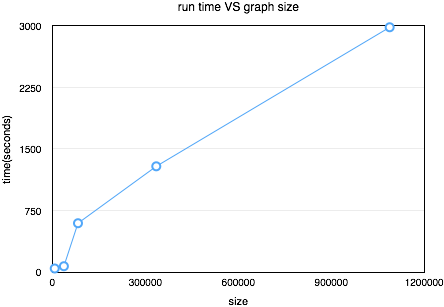
\includegraphics[width=0.8\textwidth]{FIG/t7_time.png}
\end{tabular}
\caption{Task 7: Run time VS graph size(global)}
\label{t7:globaltime}
\end{center}
\end{figure}

\begin{figure}[!htbf]
\begin{center}
\begin{tabular}{cc}
     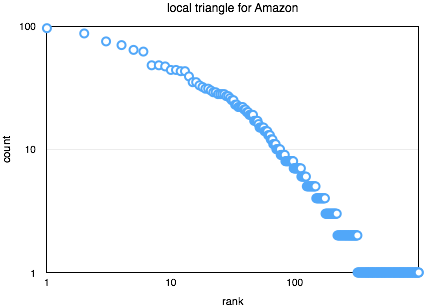
\includegraphics[width=0.4\textwidth]{FIG/t7_amazon.png} &
     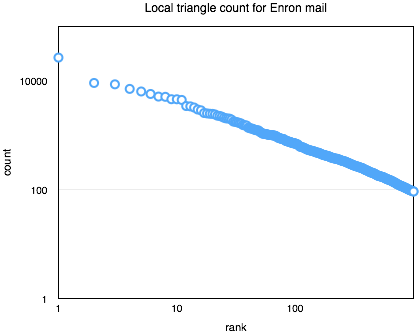
\includegraphics[width=0.4\textwidth]{FIG/t7_enron.png} \\
     (a) & (b) \\
     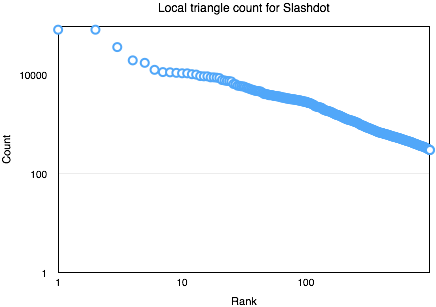
\includegraphics[width=0.4\textwidth]{FIG/t7_slashdot.png} &
     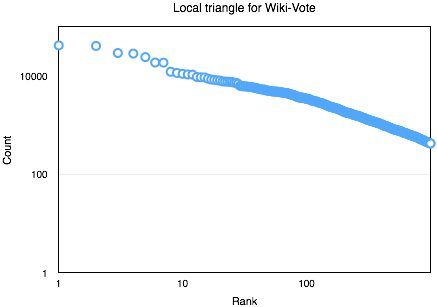
\includegraphics[width=0.4\textwidth]{FIG/t7_wikivote.png} \\
     (c) & (d) \\
     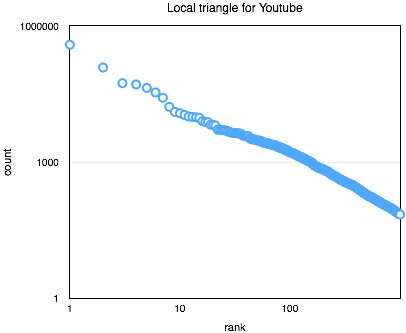
\includegraphics[width=0.4\textwidth]{FIG/t7_youtube.png} & \\
     (e)
\end{tabular}
\caption{Local triangle counting. (a) Amazon (b) Enron Mail (c) Slashdot (d) Wiki Vote (e) Youtube}
\label{t7:local}
\end{center}
\end{figure}

\subsubsection{Observation}
According to Figure \ref{t7:local}, we can see that the rank-frequency plot of local triangle count also follows power law. And we can observe that the run time grows nearly linearly with the graph size. 


\subsection{Innovative task: Shortest Path}
{\bf Proof of Correctness: } In order to prove the correctness, we conduct experiments on a small dataset that we manually constucted. 

\subsection{Innovative task: Minimum Spanning Tree}
\subsubsection{Proof of Correctness}
In order to verify the correctness of our implementation, we first run our algorithm on tiny synthetic graph with 10 nodes and 17 edges. We verified the result is correct. Then we compare our implementation against MATLAB's implementation of Minimum Spanning Tree and we get identical result for output of both implementation.

\subsubsection{Experiment on Large datasets}
Since MST algorithm require that graph is fully connected, weighted, and undirected. We can barely find such graph in Konect and SNAP project. Therefore, we generate synthetic graph of different size. We plot the runtime against graph size (number of nodes) in Figure \ref{mst:fig}. We find the run time grows near-quadratically as the number of nodes in graph. This is identical to the time complexity of Prim's Algorithm, which is $O(N^2)$.

\begin{figure}[!htbf]
\begin{center}
     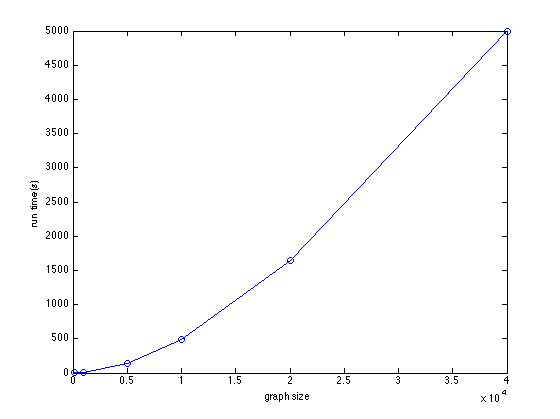
\includegraphics[width=0.8\textwidth]{FIG/mst.png} 
\caption{MST runtime plot}
\label{mst:fig}
\end{center}
\end{figure}


\begin{table}
\begin{center}
\begin{tabular}{| l | c |}
  \hline                        
  Size of WCC & Count  \\ \hline
  1 & 1384  \\ \hline
  2 & 55  \\ \hline
  3 & 1 \\ \hline
  5054 & 1 \\ \hline  
\end{tabular}
\caption{Statistics about Weakly connected components}
\label{table:wcc}
\end{center}
\end{table}

\begin{table}
\begin{center}
\begin{tabular}{| l | c |}
  \hline                        
  radius & number of vertices  \\ \hline
  0 & 1896  \\ \hline
  1 & 84  \\ \hline
  2 & 11 \\ \hline
  3 & 7 \\ \hline  
  4 & 634 \\ \hline  
  5 & 2194 \\ \hline  
  6 & 826 \\ \hline  
  7 & 117 \\ \hline  
  8 & 13 \\ \hline
  9 & 2 \\ \hline   
\end{tabular}
\caption{statistics about radius}
\label{table:radius}
\end{center} 
\end{table}

\begin{figure}[htbf]
\begin{center}
     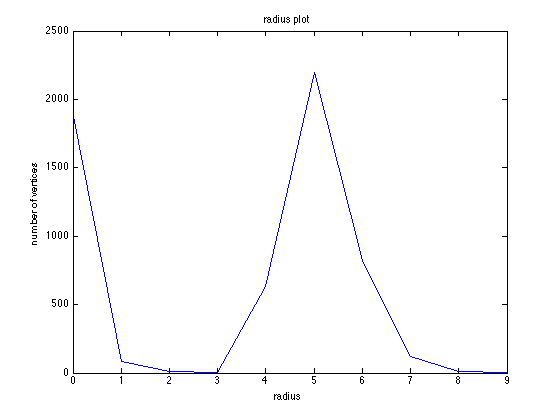
\includegraphics[width=0.6\textwidth]{FIG/radius.png}
\caption{Radius Plot}
\label{fig:radius}
\end{center}
\end{figure}

\subsection{Broad Spectrum Analysis}
We apply our proposed graph mining algorithms to several real-world graph datasets from KONECT project to find global patterns and detect strange behaviors. In the following, we'll first describe the dataest then discuss  what we observe. 

\begin{description}
	\item{{\bf Route Views\cite{konect:2013:as20000102, konect:DBLP}:}}{This is an undirected network of autonomous systems of the Internet connected with each other. Nodes are autonomous systems (AS), and edges denote communication. The network contains loops. It contains 6,474 vertices and 13,895 edges.}
	\item{{\bf DBLP\cite{konect:2013:dblp-cite, konect:DBLP}:}}{This is the citation network of DBLP, a database of scientific publications such as papers and books. Each node in the network is a publication, and each edge represents a citation of a publication by another publication. In other words, the directed edge (A to B) denotes that publication A cites publication B. Publications are allowed to cite themselves, and therefore the network contains loops. It contains 12,495 vertices and 49,793 edges.}
\end{description}

\begin{figure}[htbf]
\begin{center}
\begin{tabular}{cc}
     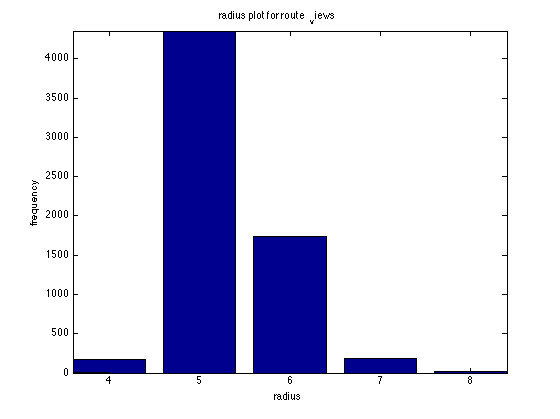
\includegraphics[width=0.4\textwidth]{FIG/route_radius.png} &
     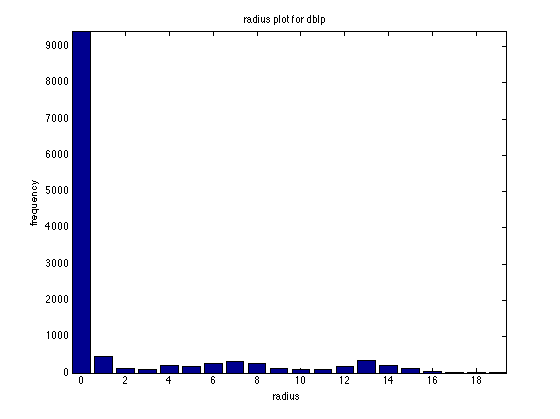
\includegraphics[width=0.4\textwidth]{FIG/dblp_radius.png} \\
    (a) & (b) 
\end{tabular}
\caption{Radius plot for Route Views (a) and Radius plot for DBLP (b)}
\label{fig:radius_plot}
\end{center}
\end{figure}

The radius plot for dataset are shown in figure \ref{fig:radius_plot}. 

From radius distribution of route views, we can see that all the vertices has radius more than 3. And since this is a connected graph (from the result we got by applying connected component algorithm), we can conclude that vertices(Autonomous Systems) with smaller radius plays a more centric role in the graph where most other vertices have direct or indirect communication (within very few hops) with. We find very few vertices with radius 4 are in the center of the graph, then most of the vertices with radius 5 are surrounding these centric vertices. Then the number of vertices decrease exponetialy as the radius grows. And finally, very few vertices (less than 20) are in the margin of the entire AS networks.  

For another graph DBLP, we observe strange behaviors. In this radius distribution, we observe that the great majority of the vertices have 0 radius, which means these papers didn't cite any other papers. We can only explain this observation by assuming all the cited papers of all those 9000 papers are not within this dataset. For other radius value, we don't observe apparent power law but rather more or less uniform distribution. However, in an exact or more complete citation graph, we should see several few popular papers pointing to each other, and has rather small radius, and most other less famous papers has longer citation path (larger radius). Therefore, we can conclude that this is a small sub-graph that don't capture the significant characteristic of a complete citation graph.




\section{Conclusions}
    \label{sec:conclusions}
    % The proposed method {\em someMETHOD}
% has the following advantages:
% \bit
% \item it gives better classification accuracy than all 10 competitors we tried
% \item its accuracy is very close to the very best competitor
%       in the {\em UCR Insect Classification Contest}.
% \item it is scalable
% \eit

In this project, we investigate the major questions discussed in graph mining. We 
explored and solved the following problems:

\begin{itemize}
    \item We summarize the importance of graph mining techniques and propose our approach
    to this problem, which is Relational Database Management System.
    \item We conduct extensive survey about 7 graph mining tasks, each team member has read
    at least six papers each for the tasks. 
    \item For task 1, we calculate degree distribution of each node and do visualization. By 
    observing the plot, we conclude that {\bf social network} data exhibits {\bf power law}, while
    this is not a general rule, for instance, Roadnet dataset doest not show power law.
    \item For task 2, we calculate the pagerank of each node in a graph, namely the importance of each
    node. By visualize the pagerank distribution in a rank-frequency plot, we again observe {\bf power law}.
    \item For task 3, we compute the weakly connected components for a graph. By observing the plot, we find
    that there is a Giant Connected Component(GCC) which contains the majority of nodes in a graph. And the frequency-size 
    plot exhibits {\bf power law}.
    \item For task 4, we calculate the radius for every node in a graph using an approximate algorithm.
    By visualizing the result as radius plot, we find that most graphs has a {\bf single-modal} or {\bf bi-modal} radius distribution. 
    \item For task 5. We tackle the problem of calculating eigenvalue of an adjacent matrix by Lanczos mathod. We 
    build a Python matrix operation library which wraps low level linear algebra operations of SQL. 
    \item For task 6. We implement the belief propagation using FABP algorithm. By conducting experiments on large datasets,
    we successfully perform {\bf semi-supervised learning} using partially available labels to inference the labels of other nodes in the graph. 
    \item For task 7. We deal with the problem of count triangle(global or local) in a graph by calculating the
    eigenvalue of the adjacent matrix. Through the rank-frequency plot of local triangle distribution, we again
    observe {\bf power law}.
    \item We finished 2 innovative tasks, namely shortest path, minimum spanning tree. 
    \item We provide proof of correctness for each task we implemented. 
\end{itemize}



\bibliography{BIB/christosref,BIB/other,BIB/siping_ref,BIB/weichen_ref}
\bibliographystyle{plain}

\newpage
\appendix
\section{Appendix}
\subsection{Labor Division}

The team performed the following tasks
\bit
\item Implementation of Task 1,2 [Wei Chen]
\item Implementation of Task 3 [Siping Ji]
\item Implementation of Task 4,6. [Siping Ji]
\item Implementation of Task 5,7. [Wei Chen]
\item Implementation of Shortest Path(Innovative). [Wei Chen]
\item Implementation of Minimum Spanning Tree. [Siping Ji]
\item Set up testing framework in travis\footnote{travis-ci.org}. [Wei Chen]
\item Data collection [Wei Chen, Siping Ji]
\item Experiments on the real data [Wei Chen, Siping Ji]
\eit

\subsection{Project Development}
All the project related activity(code, report) are managed by Github\footnote{https://www.github.com}, a collaborative development community. All tasks are mapped into \emph{issues}, each phase is a \emph{milestone}. We fork from a central repository, when we finish our assigned tasks(issue), we send a pull request to the central repository. We are responsible for code review each other's code, then merge into the central repository. It's easy to see each team member's contribution by review the history of pull request and commit. The project address is here.\footnote{https://github.com/essex405/graph-mining-rdbms}

\subsection{Plan}

\begin{center}
Phase 1\\
\begin{tabular}{|c|c|c|}
\hline
Task & Due & Member \\\hline
Task1 & 10/07/13 & Wei\\\hline
Task2 & 10/07/13 & Wei\\\hline
Task3 & 10/07/13 & Siping\\\hline
\end{tabular}
\end{center}

\begin{center}
Phase 2\\
\begin{tabular}{|c|c|c|}
\hline
Task4 & 11/05/13 & Siping\\\hline
Task5 & 11/05/13 & Wei\\\hline
Task6 & 11/05/13 & Siping\\\hline
Task7 & 11/10/13 & Wei\\\hline
Task8 & 11/10/13 & Siping\\\hline
Final & 11/20/13 & Wei, Siping\\\hline
Poster & 11/20/13 & Wei, Siping\\\hline
\end{tabular}
\end{center}

\begin{center}
Phase 3\\
\begin{tabular}{|c|c|c|}
\hline
Packaging code & 11/30/13 & Wei Chen, Siping \\ \hline
Final report & 11/30/13 & Wei Chen, Siping \\ \hline
\end{tabular}
\end{center}


\subsection{Additional Task}
In addition to the default tasks,  we plan to complete another two:  shortest path and minimum spanning tree. The detailed report please refer to {\bf Experiments}.

\subsection{Unit Tests}
The host language we use is Python, thus we plan to use its internal unit test framework\footnote{http://docs.python.org/2/library/unittest.html} as our testing module. We did unit tests for following modules:
\bit
\item Matrix Vector multiplication, abstract out the some basic matrix-vector, matrix-matrix operations. 
\item SQL user defined function bit-or
\item SQL user defined function fm-size
\eit

\newpage
\subsection{Source Code}
\subsubsection{../src/bp/bp.py}
\lstinputlisting{../src/bp/bp.py}
\subsubsection{../src/cc/assign.sql}
\lstinputlisting{../src/cc/assign.sql}
\subsubsection{../src/cc/cc.py}
\lstinputlisting{../src/cc/cc.py}
\subsubsection{../src/cc/count\_diff.sql}
\lstinputlisting{../src/cc/count_diff.sql}
\subsubsection{../src/cc/init.sql}
\lstinputlisting{../src/cc/init.sql}
\subsubsection{../src/cc/main.sql}
\lstinputlisting{../src/cc/main.sql}
\subsubsection{../src/cc/stat.sql}
\lstinputlisting{../src/cc/stat.sql}
\subsubsection{../src/cc/update.sql}
\lstinputlisting{../src/cc/update.sql}
\subsubsection{../src/common/basic\_operation.py}
\lstinputlisting{../src/common/basic_operation.py}
\subsubsection{../src/common/util.py}
\lstinputlisting{../src/common/util.py}
\subsubsection{../src/ddis/ddis.py}
\lstinputlisting{../src/ddis/ddis.py}
\subsubsection{../src/eigenvalue/eigen\_quodratic.py}
\lstinputlisting{../src/eigenvalue/eigen_quodratic.py}
\subsubsection{../src/eigenvalue/lanczos.py}
\lstinputlisting{../src/eigenvalue/lanczos.py}
\subsubsection{../src/eigenvalue/qr\_decompose.py}
\lstinputlisting{../src/eigenvalue/qr_decompose.py}
\subsubsection{../src/eigenvalue/test\_data.txt}
\lstinputlisting{../src/eigenvalue/test_data.txt}
\subsubsection{../src/generate\_appendix.sh}
\lstinputlisting{../src/generate_appendix.sh}
\subsubsection{../src/graph\_generator.py}
\lstinputlisting{../src/graph_generator.py}
\subsubsection{../src/misc/pagerank.py}
\lstinputlisting{../src/misc/pagerank.py}
\subsubsection{../src/mst/mst.py}
\lstinputlisting{../src/mst/mst.py}
\subsubsection{../src/mst/test.dat}
\lstinputlisting{../src/mst/test.dat}
\subsubsection{../src/pagerank/pagerank.py}
\lstinputlisting{../src/pagerank/pagerank.py}
\subsubsection{../src/pagerank/query.py}
\lstinputlisting{../src/pagerank/query.py}
\subsubsection{../src/radius/functions.py}
\lstinputlisting{../src/radius/functions.py}
\subsubsection{../src/radius/hop.sql}
\lstinputlisting{../src/radius/hop.sql}
\subsubsection{../src/radius/radius.py}
\lstinputlisting{../src/radius/radius.py}
\subsubsection{../src/radius/radius\_test.py}
\lstinputlisting{../src/radius/radius_test.py}
\subsubsection{../src/radius/README}
\lstinputlisting{../src/radius/README}
\subsubsection{../src/radius/utils/agg\_bit\_or.sql}
\lstinputlisting{../src/radius/utils/agg_bit_or.sql}
\subsubsection{../src/radius/utils/bit\_or.sql}
\lstinputlisting{../src/radius/utils/bit_or.sql}
\subsubsection{../src/radius/utils/fm\_assin.sql}
\lstinputlisting{../src/radius/utils/fm_assin.sql}
\subsubsection{../src/radius/utils/fm\_size.sql}
\lstinputlisting{../src/radius/utils/fm_size.sql}
\subsubsection{../src/radius/utils/functions.py}
\lstinputlisting{../src/radius/utils/functions.py}
\subsubsection{../src/radius/utils/lsb.sql}
\lstinputlisting{../src/radius/utils/lsb.sql}
\subsubsection{../src/spath/dijkstra.py}
\lstinputlisting{../src/spath/dijkstra.py}
\subsubsection{../src/test\_bp.py}
\lstinputlisting{../src/test_bp.py}
\subsubsection{../src/test\_connected\_component.py}
\lstinputlisting{../src/test_connected_component.py}
\subsubsection{../src/test\_degree\_distribution.py}
\lstinputlisting{../src/test_degree_distribution.py}
\subsubsection{../src/test\_eigenvalue.py}
\lstinputlisting{../src/test_eigenvalue.py}
\subsubsection{../src/test\_pagerank.py}
\lstinputlisting{../src/test_pagerank.py}
\subsubsection{../src/test\_radius.py}
\lstinputlisting{../src/test_radius.py}
\subsubsection{../src/test\_shortest\_path.py}
\lstinputlisting{../src/test_shortest_path.py}
\subsubsection{../src/test\_triangle.py}
\lstinputlisting{../src/test_triangle.py}
\subsubsection{../src/test\_triangle\_local.py}
\lstinputlisting{../src/test_triangle_local.py}
\subsubsection{../src/triangle/tria.py}
\lstinputlisting{../src/triangle/tria.py}


\newpage
\pagenumbering{roman}
\tableofcontents


\end{document}
